\documentclass[a4paper,12pt]{article} %{IEEEtran}
%\usepackage[slovene]{babel}
\usepackage[utf8]{inputenc}
\usepackage{graphicx}
\usepackage[T1]{fontenc}
\usepackage{lmodern}
\usepackage{url}
\usepackage{cite}
\usepackage{amsthm}
\usepackage{amssymb}
\usepackage{listings} %za pisanje kode
\usepackage{float} %za natančno specificiranje pozicije slik

\makeatletter
\newcommand{\mybox}{%
    \collectbox{%
        \setlength{\fboxsep}{1pt}%
        \fbox{\BOXCONTENT}%
    }%
}
\makeatother

\textwidth 15cm
\textheight 24cm
\oddsidemargin.5cm
\evensidemargin.5cm
\topmargin-5mm
\addtolength{\footskip}{10pt}
\pagestyle{plain}
\overfullrule=15pt


%%%%%%%%%%%%%%%%%%%%%%%%%%%%%%%%%%%%%%%%%%%%%%%%%%%%%%%%%%%%%

\begin{document}
\begin{center}
\begin{Large}
\textbf{Razvoz blaga z roboti}\\
\end{Large}
\begin{large}
Projekt pri predmetu Umetna inteligenca\\
\vspace{3mm}
\end{large}
Anže Marinko in  Ana Golob
\end{center}

\section{Opis problema}



Imamo šahovnico velikosti $n \times m$. Vsako polje na šahovnici ima lastnosti enega izmed spodnjih tipov:

\begin{itemize}

\item Pot: na tem polju se lahko nahaja robot, vendar največ en robot hkrati.

\item Skladišče: vsebuje ponudbo predstavljeno s slovarjem dobrin dobrin skupaj z njihovimi količinami. Roboti se ne morejo gibati po tem polju.

\item Trg: vsebuje povpraševanje predstavljeno s slovarjem dobrin skupaj z njihovimi količinami. Roboti se ne morejo gibati po tem polju.

\end{itemize}

Na šahovnici imamo $k$ robotov. Vsak robot ima določeno maksimalno količino dobrin, ki jih lahko nosi. Robot se lahko premika po poljih tipa pot v smereh levo, desno, gor in dol. Robot lahko prevzame različne količine blaga iz skladišča, ki se nahaja na sosednem polju. Poleg tega lahko odloži blago, ki ga nosi na trgu, ki se nahaja na sosednjem polju. Roboti se lahko premikajo sočasno.\vspace{3mm}

\framebox{
\parbox[t][1.5cm]{13cm}{
\addvspace{0.2cm} \centering 

CILJ: Poiskati čim kraše zaporedje potez (ena poteza je lahko sestavljena iz več sočasnih premikov robotov), 
ki so potrebne, da zadostimo vsemu povpraševanju na trgih.
}
}\\
\vspace{2mm}

Pri tem so različne konkretne realizacije zgoraj opisanih problemov generirane naključno. Algoritem z nespremenjenimi parametri so bili preizkušeni na večih različnih tako dobljenih primerih.

\section{Hevristika A*}

Želimo optimistično hevristično funkcijo, da bi si zagotovili najkrajšo rešitev, hkrati, pa se želimo čim bolje približati točnemu najmanjšemu številu preostalih potez do konca.

Naj bosta $D = \lbrace D_i; \forall i\in B\rbrace$ slovar ponudb in $S = \lbrace S_i; \forall i\in B\rbrace$ slovar povpraševanja,
kjer $D_i$ seznam skladišč in robotov ter $S_i$ seznam trgov s  ponudbo ali povpraševanjem po blagu $i$ in je $B$ množica vrst blaga. Naj bo $m$ največja nosilnost enega robota, $r$ število robotov, $d_1(s,d) = |s_x-d_x|+|s_y-d_y|$ razdalja med skladiščem $d$ in trgom $s$ ter $s_q$ potrebna količina določenega blaga na trgu $s$.

Hevristično funkcijo definiramo kot

$$f(S,D) = \frac{1}{r}\sum_{i\in B}\sum_{s\in S_i}\lceil \frac{d_1(s,d^\ast(s,i))}{m} s_q\rceil,$$
kjer je $d^\ast(s,i)\in D$ trgu $s$ v 1-normi najbližje skladišče ali robot z blagom $i$.

Funkcija je očitno optimistična, saj je lahko kvečjemu enaka dejanskemu minimumu, saj ima morda kakšen robot manj prostora od $m$, ker morda ni mogoče priti od skladišča do trga po najkrajši poti med njima, ker morda v najbližjem skladišču ni dovolj blaga in ker se bo morda moral še vračati po isti poti nazaj oz. je všteta le pot od skladišč do trgov in ne tudi obratno. Lahko bi imeli tudi manj optimistično funkcijo, a bi postal izračun vrednosti že dosti bolj kompleksen, če bi upoštevali tudi neke posplošitve, ki jih ta model predpostavlja (vsi roboti enaki ipd.).

\section{Q learning algoritem}

Implementiran je tudi Q learning algoritem, vendar je v primerjavi z algoritmom A* precej počasnejši, poleg tega ne zagotavlja optimalne rešitve. Glavna težava pri doseganju optimalnih rezultatov je bila, da je funkcija nagrajevanja, ki doseže optimalne rezultate, različna za različne primere.

\section{Analiza rezultatov z A* algoritmom}

Algoritem je bil preizkušen na naključno definiranih testnih primerih. Med primeri so se spreminjali parametri: dimenzija šahovnice, število robotov, število trgov, število skladišč, število različnih vrst blaga in skupna količina povpraševanja po blagu. Razlikovala se je tudi razporeditev različnih polj po šahovnici, pri čemer so bili izločeni nerešljivi primeri. Analiziran je bil vpliv naštetih parametrov na spremembo časa izvajanja.

Tekom testiranja se je izkazalo, da ima največji vpliv na čas izvajanja algoritma število robotov. Kar je smiselno, saj se lahko roboti premikajo sočasno in zato večje število robotov zelo močno  poveča število možnih potez v določenem stanju. Izmed preostalih parametrov je imela opatzen vpliv tudi količina blaga, ki ga je potrebno pripeljati na trge. Spodnji graf prikazuje vpliv omenjenih parametrov na čas izvajanja.

\begin{figure}[H]
\begin{center}
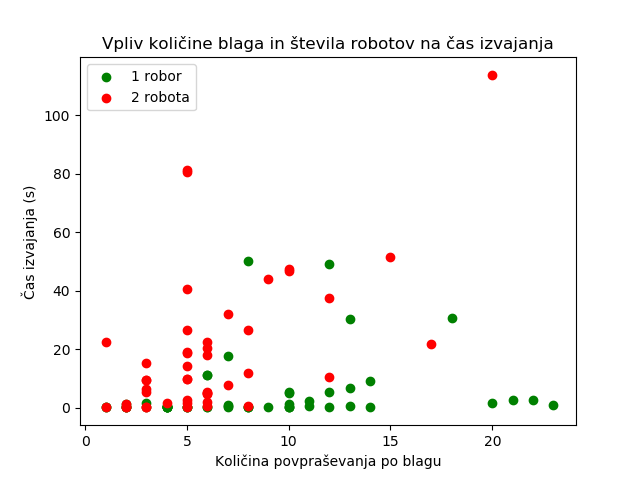
\includegraphics[width=9.8cm]{cas_izvajanja.png}
\end{center}
\end{figure} 


\end{document}
